\documentclass[prl,showpacs,superscriptaddress,twocolumn,longbibliography]{revtex4-1}

\usepackage{hyperref}
\usepackage{url}
\usepackage{color}
\usepackage[usenames,dvipsnames]{xcolor}
\usepackage{amsmath,amsthm,amssymb}
\usepackage{graphicx}
\usepackage{bm}% bold math
\usepackage[all]{xy} 
\usepackage{verbatim}
\usepackage{braket}
\usepackage{mathtools}
\usepackage{bm}
\usepackage{tikz}
\usepackage{xcolor}
\usepackage{float}
%\usepackage{tabstackengine}
\usepackage{enumerate}   


\begin{document}

\author{Erin Aho}
\author{Albert Nyarko-Agyei}
\author{Soham Talukdar}

\title{Using Feature Selection to Identify Features that are Most Important to Species Richness in Butterflies}

\begin{abstract}
Butterflies are an important taxa, both ecologically and culturally, but populations have been declining globally despite conservation efforts. To improve understanding of where to focus conservation efforts we aim to identify the features that are the most informative of an area's species richness.
The species count of butterflies in 45 broad regions was analysed. Based on existing research, we decided on a set of 28 features, both bioclimatic and anthropogenic, which are known to affect species richness. After researching current feature selection methods, we decided to use Joint Mutual Information (JMI) as our selection criterion, due to the high amount of mutual information in many of our features, and the strong performance JMI has been shown to have for small sample sizes. After performing feature selection on our dataset using JMI, we were able to identify that the most informative set of 5 features is made up of: temperature seasonality, precipitation in the driest month, precipitation in the warmest quarter, max temperature in the warmest month, and the mean diurnal range . We discuss possible limitations of our approach, and areas further research is needed in order to better understand butterfly species richness.
\end{abstract}

\maketitle

\noindent {\bf\em Introduction.--}
Butterflies (Lepidoptera: Rhopalocera) are among the most familiar group of all insects, approximately 17,200 species worldwide\cite{shields_world_1989}. They have been prominently featured in cultural imagery going back at least two millennia.\cite{Dicke2000}, and historically they have played an important part in developing our understanding of biodiversity\cite{levin_butterflies_2001}. 

Butterflies also have a vital role in their ecosystems, where they act as a pollinator, helping plants to reproduce and increasing floral genetic variation\cite{ghazanfar_butterflies_2016}.

Their cultural and ecological importance makes it especially worrying that, despite conservation efforts, butterfly populations have been declining rapidly alongside most insect groups worldwide \cite{Wagner2021}. While it is known that this unprecedented rate of biodiversity loss is tied with human activities, such as deforestation and climate change\cite{white_human_2007, montgomery_is_2020, clark_effects_2007}, there has been limited success in predicting where best to focus future conservation efforts. By finding which factors provide the most information about butterfly species richness, we aim to reduce this knowledge gap and help direct conservation efforts to where they are most needed.

\noindent {\bf Existing understanding.--}
Species richness (i.e., the number of species occurring in a given area) is commonly used as a health descriptor for a community, as it combines many relevant ecological features such as environmental stability, ecosystem productivity, and biological factors\cite{Park2003}.

One feature which is sure to impact the number of species in a given region is the region's area. Regarding how the number of species in a region varies with the area of the region, it has been observed that log(species count) correlates with log(area)\cite{connor_2001_sar}. Connor \& McCoy (1979) discussed two main hypotheses explaining species-area relationships (SAR):(i) the habitat diversity hypothesis; and (ii) the demographic process hypothesis. The first hypothesis states that larger areas are more likely to contain more habitat types, which could support a greater diversity of species. In contrast, the demographic explanation incorporates the dynamic processes of dispersal, colonization, speciation and extinction at multiple spatial scales. Larger areas have higher probabilities of colonization and speciation and lower probabilities of extinction, fostering higher diversity\cite{drakare_impint_2006}.  Investigating these hypotheses is beyond the scope of this paper, and while these hypotheses may disagree on the exact mechanism that drive the SAR, they agree $log(species \: count)$ correlates with $log(area)$, which is a key result we will make use of in our methodology.

Many factors which influence species viability can vary considerably even within small distances\cite{john_wiley__sons_ltd_species_2007}. It is well known that total available energy (most commonly solar energy flux) is an important factor for the overall biodiversity in a region\cite{hawkins_energy_2003, currie_energy_1991}. For butterflies in particular, changes in volume of rainfall in local micro-climates has been shown to strongly affect the population of several species of butterflies\cite{Haneda2019}. It has also been shown that Butterfly communities follow Rapoport's Rule, and show a strong elevational gradient in species richness\cite{fleishman_empirical_1998, Arturo}. 

Several studies show that agricultural land use can affect both habitat suitability and availability of species who would live in grasslands\cite{smith}. Urbanization is one of the most important causes of natural habitat loss and fragmentation, and is linked to decreased plant species diversity, reduced water quality, and increased air and soil pollution, which in turn can cause species diversity decline\cite{smith,Tzortzakaki2019}. 
Modern ecological research commonly investigates anthropogenic causes of biodiversity loss like urbanisation, deforestation, and global environmental change, with the aim of better understanding how human activity is affecting our planet so that we might mitigate our harmful impacts\cite{hill_responses_2002, munguira_conservation_1995, white_human_2007, sanchez-bayo_worldwide_2019}. Against this background, understanding the relationship between species richness and environmental factors is particularly important. 

Exactly which features are most important to species richness is not well understood, and differs for each taxa. We aim to help shrink this gap in information for butterflies by finding which features are the most important to track so that we can better understand how the impacts of anthropogenic habitat disruption will affect butterflies moving forward. We have thus created a broad set of features based on the factors which are important to biodiversity, informed by our discussion above, and aim to find the most informative features for Butterflies specifically.


\noindent 

{\bf\em Method.--}We were provided with a set of 45 regions, and the number of species found in each. We generated a dataset by taking the mean across our regions for each feature, using open-source GIS tools.

Based on the work in Species-Area relationships by Connor et al\cite{connor_2001_sar}, we created our target variable from the given data by taking $log(species \: count)/log(area)$, which gives us an estimator for species richness that is not dependent on the area of a region. Based on the studies discussed, we identified the importance of accounting for climatic variation, elevation, available energy, and human influences.  To account for climatic variability, we used the unitary 19 bioclimatic indices which account for the main climate-based physiological constraints for biodiversity\cite{hijmans_very_2005}. Our elevation, net solar flux and land coverage data are from the NASA Near Earth Observatory. We created our feature variables using open source GIS tools\cite{QGIS_software} to calculate zonal statistics, or a zonal histogram in the case of land coverage data over open source vectors for each region\cite{natural_earth_vectors, gadm_vectors, taman_kinbalu_pp, calakmul_pp}, and rasters for each of the features we wanted to investigate. The output from the GIS feature extraction, as well as any preprocessing done before inputting the features into our model, is available on Github \footnote{https://github.com/E-Aho/Butterfly-Modeling}. The full list of features used, and the sources for the rasters, is given in Appendix A.

As we are aiming to create a set of features that are easily interpreted and applied to new data, we decided to use feature selection over principal component analysis (PCA). Within feature selection, we made use of a filter method instead of a wrapper method to limit the risk of over-fitting, which could be quite prominent due to the large number of features in total (28) when compared to the total number of regions we had observations for (45).

Choosing a selection criterion is non-trivial, and decades of trying theoretical and heuristic approaches has produced a large number of options. Brown et al\cite{Brown2012} found that Joint Mutual Information (JMI)\cite{yang_data_1999} had the best overall performance in their framework across a number of small sample size datasets. Given our small dataset, we decided to use JMI as our selection criterion.

JMI is an extension of the Mutual Information Feature Selection (MIFS) criterion, proposed by Battiti in 1994:

\[ 
    J_{MIFS}(X_k) = I(X_k;Y) - \beta \sum_{X_j\in S} I(X_k;X_j)
\]

where S is the set of currently selected features, $X_k$ is a feature to select, $Y$ is our target variable, I denotes the information shared,  and $ \beta $ is a hyperparameter, which must be set experimentally. Using $\beta  = 0 $ would be equivalent to treating each feature as fully independent, and a larger value places focuses more on reducing inter-feature dependencies in the selected data. 

Yang and Moody (1999) and Meyer et al. (2008) proposed JMI in an effort to reduce the need to train hyperparameters, while still minimising redundancy in a selected feature set\cite{Brown2012}. The JMI score for a feature $X_k$ given an already selected set of features $S$ is:
\[ 
    J_{JMI}(X_k) =  \sum_{X_j\in S} I(X_kX_j;Y)
\]

One major difficulty in implementing a information based feature selection method is that entropy (and therefore information) for continuous variables is not as simple to calculate as it is for discrete variables. B. Ross\cite{Ross2014} and D. Homola \cite{Homola2016} championed a kNN-based approach to estimating shared information, advancing work done by Kraskov et al in 2004\cite{kraskov_estimating_2004}. This method avoids needing to bin continuous data by using k-nearest neighbour distances to estimate entropy instead, which we made use of in our implementation. For further details on how our implementation works, the code is available on Github \footnote{https://github.com/E-Aho/Butterfly-Modeling}.


\noindent {\bf\em Results.--}\begin{center}\begin{tabular}{||c c||}
 \hline
First 10 Features & Information Gain \\
 \hline\hline
 Mean temperature seasonality & 0.801\\ 
 \hline
 Mean precipitation of driest month & 1.04\\
  \hline
 Mean precipitation of warmest quarter &  1.01\\
 \hline
 Mean max temperature of warmest month &  0.957\\
 \hline
 Mean diurnal range & 0.949\\
 \hline
 Precipitation of wettest quarter & 0.913\\
 \hline
 Annual precipitation & 0.876\\
 \hline
 Latitude & 0.861\\
 \hline
 Annual mean Temperature & 0.854\\
 \hline 
 Annual insolation & 0.848\\[1ex]
\hline
\end{tabular}
\end{center}

The result of the JMI feature selection algorithm highlighted a set of features that have an optimal information gain with the target variable of this paper, $log(species \: count)/log(area)$. The mean temperature seasonality was the first feature selected by the algorithm. This means that when we took each feature and the target variable, this feature had the highest amount of information gain. The full table of all sequentially selected features and their information gains are given in Appendix B.

\begin{center}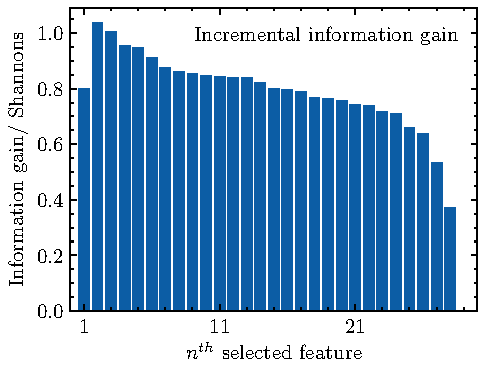
\includegraphics[width=240pt]{Features.pdf}\end{center}

\noindent {\bf\em Discussion.--}
As we can see from the above plot, adding the second feature (precipitation in the driest month) added significantly more information than the first variable did alone. This shows that seasonality and the precipitation in the driest month together hold extra information about our target variable than either did separately. Precipitation is also known to be one of the most important environmental factors for butterflies\cite{rueda-m_environmental_2021}, so seeing seasonal precipitation features be among the most informative in our dataset make sense.

After adding the second feature, successive additions result in less information gain. This is indicative of increasing amounts of redundancy in our dataset. It should be noted that each feature is still increasing the total amount of information within our selected set, but that some of the information is already accounted for in other variables already selected (e.g mean temperature in the summer has a large amount of redundancy with annual max temperature).

It is interesting to consider the correlation of the variables and the species density along with their order of selection. From the original list of features, the mean minimum temperature of the coldest month had the highest correlation with the species density, but it was selected second last. The next highest correlated feature was mean annual precipitation, which was selected 7th by our algorithm. This emphasises the difference between information gain and correlation, as the most informative feature may not be correlated well if the relationship is non-linear.

Among the features we looked at which were intended to investigate anthropogenic effects (PM 2.5 concentration \& land usage percentages), PM 2.5 was the most informative, and was selected 17th. While it is interesting to note that our anthropogenic variables were not found to be particularly informative, this may be an artefact of our methodology. Due to the majority of our regions being large in area (country sized), and the nature of local human effects typically being short ranged (habitat destruction, air pollution, etc) \cite{he_urban_2014}, it is likely climatological variables were more important at the wide scale of our regions. Further research is needed at with smaller scaled regions, and a larger number of observations, to better identify how butterfly species richness interacts with these features. 

However we should also note that wide scale climate change brought about by human actions has already been shown to affect precipitation and temperature patterns\cite{trenberth_changes_2011, ashton_effects_2009}, and that butterflies in particular are sensitive to changes in temperature extremes that relate to seasonality\cite{bauerfeind_simulating_2014}. Given that our most informative features on butterfly species richness are all rapidly changing year on year as a result of anthropogenic climate change\cite{loarie_velocity_2009}, it is clear that butterfly species richness will be sensitive to future changes in these features. 

A further limitation of our method is that we could not account for human biases in data collection. If more time is spent researching butterflies in a given area, then it is likely that more species will be found. While butterflies are one of the most studied taxa, there are predicted to still be many undiscovered species, particularly in remote areas. In turn, the robustness of species counting methods, such as counting along a transect, are also questioned by Kevin Gross et al\cite{gross_robustness_2007}. While it is hard to account for these factors, the high uncertainty in the true number of species in an area may limit the accuracy of our results.

One must also consider the flaws in the JMI algorithm. Critics of the JMI algorithm raise that it is a greedy algorithm, which selects a locally optimal feature at each stage. This will often result in groups of features which have the highest mutual information with the target variable, but as noted by Gao et al, this method does not guarantee a globally optimal solution\cite{gao_variational_2016}.  A further study could implement JMIM, an adaptation of the JMI algorithm proposed by Bennasar et al\cite{bennasar_feature_2015}, which tackles this issue by conducting more searches on combinations of features and compare the findings to our results.

An interestingly unimportant feature is that of the Island boolean tag, which did not show significant information gains, being the last selected feature, and having an information gain of just 0.373 shannons, compared to 0.533 shannons for the penultimate feature. This follows the findings of Kalmar and Currie in Avian species\cite{kalmar_unified_2007}. Kalmar and Currie found that most variation in species density is not context-specific, and varied similarly on continents and islands according to the same bioclimatic indices. Our findings seem to agree, and find that whether an area is an island or not does not add significant information to the dataset, and so is not particularly relevant to the species richness in butterflies.

\noindent {\bf\em Conclusion.--}
Overall, we have been successful in reducing the original 28 features to a small subset of informative features for butterfly species richness. These findings can be used to help identify areas to focus conservation efforts on. However, they highlight that the list of features that affect butterfly richness is complex and that many connections exist between these variables. We hope that these findings might help inform conservation efforts by combining them with climatic predictions to identify areas that are most at risk of biodiversity loss in butterflies.

\bibliography{Bibliography}
\bibliographystyle{apsrev4-1}

\onecolumngrid
\appendix

\section{Appendix A: Features Used} \label{appendix:raw}
The 28 features examined in our method were the following:
\begin{itemize}
\item Latitude
\item Island (boolean referring to if the region is an island or not)
\item Bioclimatic Variables (averaged across region)\cite{fick_worldclim_2017}:
\begin{enumerate}
	\item Annual Mean Temperature
	\item Mean Diurnal Range
	\item Isothermality (i.e relative scale of temperature change from day/night to temperature change across year)
	\item Temperature Seasonality
	\item Maximum temperature of warmest month
	\item Minimum temperature of coldest month
	\item Temperature annual range
	\item Mean temperature of wettest quarter
	\item Mean temperature of driest quarter
	\item Mean temperature of warmest quarter
	\item Mean temperature of coldest quarter
	\item Annual precipitation
	\item Precipitation of wettest month
	\item Precipitation of driest month
	\item Precipitation Seasonality
	\item Precipitation of wettest quarter
	\item Precipitation of driest quarter
	\item Precipitation of warmest quarter
	\item Precipitation of coldest quarter
\end{enumerate}
\item Total Annual Insolation, Dec 2020 - Nov 2021\cite{nasa_insol}
\item Annual Net Flux, Dec 2020 - Nov 2021\cite{nasa_netflux}
\item Percent Urbanisation, defined as percent land coverage that is characterized as:
\begin{itemize}
	\item Urban and Built Up\cite{nasa_landcov}
\end{itemize}
\item Percent Developed, defined as percent land coverage that belongs to any of:
\begin{itemize}
	\item Cropland
	\item Urban and Built up
	\item Croplands and Vegatation\cite{nasa_landcov}
\end{itemize}
\item Percent Naturally Vegetated, defined as percent land coverage that belongs to any of:
\begin{itemize}
	\item Evergreen Needleleaf Forest
	\item Evergreen Broadleaf Forest
	\item Deciduous Needleleaf Forest
	\item Deciduous Broadleaf Forest
	\item Mixed Forest
	\item Closed Shrublands
	\item Open Shrublands
	\item Woody Savannas
	\item Savannas
	\item Grasslands
	\item Permanent Wetlands\cite{nasa_landcov}
\end{itemize}
\item Particulate Matter $<$ 2.5~{\textmu}m \cite{van_donkelaar_global_2016}
\item Elevation\cite{nasa_srtm}
\end{itemize}

\section{Appendix B: Full Results Table} \label{appendix:results}
\noindent {\bf\em Results.--} 
\begin{center}\begin{tabular}{||c c||}
 \hline
Sequential features selected & Information Gain $/$ shannons \\
 \hline\hline
 Mean temperature seasonality & 0.801\\ 
 \hline
 Mean precipitation of driest month & 1.04\\
 \hline
 Mean precipitation of warmest quarter &  1.01\\
 \hline
 Mean max temperature of warmest month &  0.957\\
 \hline
 Mean diurnal temperature range & 0.949\\
 \hline
 Precipitation of wettest quarter & 0.913\\
 \hline
 Annual precipitation & 0.876\\
 \hline
 Latitude & 0.861\\
 \hline
 Annual mean Temperature & 0.854\\
 \hline 
 Annual insolation & 0.848\\ 
 \hline
 Isothermality & 0.845\\
 \hline
 Temperature annual range & 0.839\\
 \hline
 Mean temperature of wettest quarter & 0.839\\
 \hline
 Precipitation of driest quarter & 0.823\\
 \hline
 Mean temperature of driest quarter & 0.802\\
 \hline
 Precipitation of wettest month & 0.798\\
 \hline
 PM 2.5 Concentration & 0.789\\
 \hline
 Precipitation seasonality & 0.767\\
 \hline
 Net Flux & 0.764\\
 \hline
 Percent Developed & 0.758\\
 \hline
 Precipitation of coldest quarter & 0.743\\
 \hline
 Mean temperature of coldest quarter & 0.739\\
 \hline
 Mean temperature of warmest quarter & 0.718\\
 \hline
 Percent Urbanized & 0.711\\
 \hline
 Elevation & 0.661\\
 \hline
 Percent Naturally Vegetated & 0.639\\
 \hline
 Minimum temperature of coldest month & 0.533\\
 \hline
 Island & 0.373\\[1ex]
 \hline
 
\end{tabular}
\end{center}

\end{document}
